\documentclass[preprint,authoryear,12pt]{elsarticle}
\usepackage{graphicx, color}
%% maxwidth is the original width if it is less than linewidth
%% otherwise use linewidth (to make sure the graphics do not exceed the margin)
\makeatletter
\def\maxwidth{ %
  \ifdim\Gin@nat@width>\linewidth
    \linewidth
  \else
    \Gin@nat@width
  \fi
}
\makeatother
\definecolor{fgcolor}{rgb}{0.2, 0.2, 0.2}
\newcommand{\hlnumber}[1]{\textcolor[rgb]{0,0,0}{#1}}%
\newcommand{\hlfunctioncall}[1]{\textcolor[rgb]{0.501960784313725,0,0.329411764705882}{\textbf{#1}}}%
\newcommand{\hlstring}[1]{\textcolor[rgb]{0.6,0.6,1}{#1}}%
\newcommand{\hlkeyword}[1]{\textcolor[rgb]{0,0,0}{\textbf{#1}}}%
\newcommand{\hlargument}[1]{\textcolor[rgb]{0.690196078431373,0.250980392156863,0.0196078431372549}{#1}}%
\newcommand{\hlcomment}[1]{\textcolor[rgb]{0.180392156862745,0.6,0.341176470588235}{#1}}%
\newcommand{\hlroxygencomment}[1]{\textcolor[rgb]{0.43921568627451,0.47843137254902,0.701960784313725}{#1}}%
\newcommand{\hlformalargs}[1]{\textcolor[rgb]{0.690196078431373,0.250980392156863,0.0196078431372549}{#1}}%
\newcommand{\hleqformalargs}[1]{\textcolor[rgb]{0.690196078431373,0.250980392156863,0.0196078431372549}{#1}}%
\newcommand{\hlassignement}[1]{\textcolor[rgb]{0,0,0}{\textbf{#1}}}%
\newcommand{\hlpackage}[1]{\textcolor[rgb]{0.588235294117647,0.709803921568627,0.145098039215686}{#1}}%
\newcommand{\hlslot}[1]{\textit{#1}}%
\newcommand{\hlsymbol}[1]{\textcolor[rgb]{0,0,0}{#1}}%
\newcommand{\hlprompt}[1]{\textcolor[rgb]{0.2,0.2,0.2}{#1}}%

\usepackage{framed}
\makeatletter
\newenvironment{kframe}{%
 \def\at@end@of@kframe{}%
 \ifinner\ifhmode%
  \def\at@end@of@kframe{\end{minipage}}%
  \begin{minipage}{\columnwidth}%
 \fi\fi%
 \def\FrameCommand##1{\hskip\@totalleftmargin \hskip-\fboxsep
 \colorbox{shadecolor}{##1}\hskip-\fboxsep
     % There is no \\@totalrightmargin, so:
     \hskip-\linewidth \hskip-\@totalleftmargin \hskip\columnwidth}%
 \MakeFramed {\advance\hsize-\width
   \@totalleftmargin\z@ \linewidth\hsize
   \@setminipage}}%
 {\par\unskip\endMakeFramed%
 \at@end@of@kframe}
\makeatother

\definecolor{shadecolor}{rgb}{.97, .97, .97}
\definecolor{messagecolor}{rgb}{0, 0, 0}
\definecolor{warningcolor}{rgb}{1, 0, 1}
\definecolor{errorcolor}{rgb}{1, 0, 0}
\newenvironment{knitrout}{}{} % an empty environment to be redefined in TeX
\usepackage{alltt}
\usepackage{amsfonts,xcolor,verbatim}
\usepackage{amssymb}
\usepackage{amsmath}
\newcommand{\X}{\mathrm{X}}
\newcommand{\Xh}{\hat{\mathrm{X}}}
\newcommand{\transpose}{^\mathrm{T}}
\usepackage{geometry}
\usepackage{url}
\newcommand{\argmax}{\operatornamewithlimits{argmax}}
\newcommand{\argmin}{\operatornamewithlimits{argmin}}



\begin{document}




\title{Sparse Canonical Correlation Analysis Relates Network-level Atrophy 
to Multivariate Cognitive Measures in a Neurodegenerative Population}
\author{Brian B. Avants}
\begin{abstract}
This study establishes that sparse canonical correlation analysis (SCCAN) identifies generalizable, structural MRI-derived cortical networks that relate to five distinct categories of cognition.  We obtain multivariate psychometrics from the domain-specific sub-scales of the Philadelphia Brief Assessment of Cognition (PBAC).  By using a training and separate testing stage, we find that PBAC-defined cognitive domains of language, visuospatial functioning, episodic memory, executive control, and social functioning correlate with unique and distributed areas of gray matter (GM).  In contrast, a parallel univariate framework fails to identify, from the training data, regions that are also significant in the left-out test dataset. The cohort includes 164 patients with Alzheimer's disease, behavioral-variant frontotemporal dementia, semantic variant primary progressive aphasia, non-fluent/agrammatic primary progressive aphasia, or corticobasal syndrome.  The analysis is implemented with open-source software for which we provide examples in the text.  In conclusion, we show that multivariate techniques identify biologically-plausible brain regions supporting specific cognitive domains.  The findings are identified in training data and confirmed in test data. 
\end{abstract}
\begin{keyword}
Alzheimer disease; frontotemporal lobar degeneration; Philadelphia Brief Assessment of Cognition, PBAC, MRI, sparse canonical correlation analysis.
\end{keyword}
\maketitle

% \citet{Norman2006}

\section{Introduction} 
Multivariate methods have advantages over univariate methods in genomics \citet{Parkhomenko2009,LeFloch2012,Hibar2011}, pattern recognition \citet{Bishop1995,roberts_parametric_1997,Tipping2001} and neuroimaging \citet{McIntosh1996,DeMartino2008,Fan2008,Tosun2012,Shamy2011} due to the high dimensionality and latent structure within these types of datasets.  Various forms of multivariate pattern analysis (MVPA) \citet{Norman2006,Habeck2008,Hanke2009,Kloppel2008681,Stonnington2010} are frequently used in (often functional) magnetic resonance imaging (MRI) studies to increase detection power  \citet{McIntosh1996,Norman2006,OToole2007,Yamashita2008}.  Recently, multivariate analysis of structural MRI has gained more attention \citet{Ryali2010,Grosenick2013,Sabuncu2011}.  The large majority of these techniques relate a multivariate pattern to a univariate outcome.  

Modern datasets allow the opportunity to relate two independent multivariate patterns.  Neuroimaging and psychometric batteries describe cognition and the brain itself, respectively, with a matrix of quantitative measurements.  These types of datasets may be analyzed with methods such as canonical correlation analysis (CCA) \citet{cherry} which is closely related to multivariate regression and partial least squares \citet{Sun2009}.  Partial least squares (PLS), without sparseness, has been used for several years in multivariate brain mapping studies \citet{McIntosh1996,Leibovitch1999,Lin2003,Addis2004a,Chen2009a}.  Ridge and related penalties allow these methods to be applied even when the number of subjects is far fewer than the number of measurements \citet{Nestor2002}.  However, a caveat of these approaches is that the resulting solution vectors have global extent i.e. cover the entire brain with basis vectors that are non-zero and may have both positive and negative values.  Traditional approaches are more clearly directional: a long neurological history is founded on relating behavioral deficits (losses) associated with destruction of brain tissue by stroke or related disorders.  Perhaps the most famous example is H.M.  This epilepsy patient lacked the ability to form new memories after anterior temporal lobe resection.  That is, loss of a specific part of the brain resulted in a specific deficit.  

Tools such as independent component analysis and principal components analysis (PCA) \citet{mansfield_analytic_1977,comon_independent_1994,yeung_principal_2001,Borroni2012,Shamy2011} increase power by efficiently describing data.  However, PCA solutions provide signed basis vectors with global support and therefore lose the specificity of classical region of interest approaches or lesion studies.  Sparse multivariate methods have advantages of interpretability \citet{lee_learning_1999,Suykens2002} and, potentially, improved generalizability \citet{elad_why_2006,Zhang2008,Yamashita2008,Ryali2010,zibulevsky_l1-l2_2010}.  In this paper, we use the cognitive variance induced by a spectrum of neurodegenerative conditions to examine how new, sparse multivariate analysis techniques more powerfully reveal relationships between brain and behavior.  At the same time, sparse methods achieve a degree of specificity that cannot naturally be obtained by dimensionality reduction tools such as PCA \citet{lee_learning_1999}.  Here, we apply sparse multivariate methods to find cortical networks that vary with cognition in a mixed group composed of controls and phenotypes related to Alzheimer's disease (AD) and Frontotemporal lobar degeneration (FTLD) pathology.

Like AD, FTLD is a progressive neurodegenerative condition that is accompanied by changes in behavior.  Unlike AD, which typically presents atrophy in the precuneus and temporal lobes, FTLD's pathology occurs more frequently in frontal and temporal lobes\citet{Rabinovici2007,Whitwell2007d}.  FTLD phenotypes include patients with a disorder of social comportment and executive functioning (bvFTD); a non-fluent/agrammatic variant of primary progressive aphasia (naPPA), also known as progressive non-fluent aphasia; a semantic variant of primary progressive aphasia (svPPA), also known as semantic dementia; and corticobasal syndrome (CBS).  A common test for cognitive deficits in dementia is the Mini-Mental State Examination \citet{Hill1995}. However, the MMSE does not assess the behavioral and cognitive deficits associated with FTLD \citet{Hutchinson2007}.  Other tests have been developed to screen and compare patients with dementia syndromes, including the Frontal Assessment Battery \citet{Dubois2000} (FAB); the Addenbrooke Cognitive Examination \citet{Galton2005} (ACE); and the Montreal Cognitive Assessment (MoCA) \citet{Nasreddine2005}.

The Philadelphia Brief Assessment of Cognition \citet{Libon2007,libon_philadelphia_2011} (PBAC) provides an economical means to screen and assess important domains of cognitive and behavioral impairment associated with AD and FTLD spectrum phenotypes.  The PBAC requires about 12 minutes for administration and scoring.  An important component of the PBAC is the construction of sub-scales designed to assess specific cognitive and behavioral/comportment deficits that typify AD and FTLD syndromes, including executive/working memory, language, visuospatial/constructional skills, verbal/visual episodic memory, and behavior/social comportment.  Dementia severity is assessed by summing all PBAC sub-scales.  Recent research with the PBAC has demonstrated that AD and FTLD patients present with specific areas of impairment on sub-scales that correspond to phenotypic syndromes \citet{libon_philadelphia_2011} \textcolor{black}{i.e. clinical diagnosis.}

The current study extends previous research with the PBAC \citet{libon_philadelphia_2011} by examining the gray matter neuroimaging correlates of PBAC's cognitive and social measurements in a large number of AD and FTLD patients.  \textcolor{black}{From a neurological perspective, the purpose, here, is to use the variance within these patients to assess brain and behavior relationships across multiple behavioral loci, as opposed to diagnosis.  From a technical perspective, the goal is to contrast univariate and multivariate techniques.}  To test the hypothesis that PBAC indirectly measures the integrity of different cortical networks (versus individual voxels), we employ a new data-driven machine learning technique, sparse canonical correlation analysis for neuroimaging (SCCAN), to associate high-dimensional imaging measurements with the full information provided by a multivariate psychometric battery such as PBAC.  Specifically, this approach allows an optimal weighting of psychometric sub-scales (as opposed to averaging their values) such that the relationship with neuroimaging is maximized.  At the same time, SCCAN optimizes and selects regions of gray matter (GM) to maximize correlation with psychometrics.  This results in a set of gray matter regions that may be interpreted as the network most-associated with the given psychometric domain.  SCCA previously identified covariation between GM and diffusion tensor imaging white matter (WM) changes that optimally discriminate between CSF- and autopsy-defined patients with AD and FTLD \citet{Avants2010b}.  The purpose of the current research is to test the hypothesis that SCCAN may employ individual PBAC sub-scales to extract GM networks that are reproducibly associated with variation in cognition.  This would provide additional criterion validity for both the PBAC and multivariate techniques such as SCCAN, in contrast to univariate techniques, and establish a novel strategy for performing multivariate analyses of brain and behavior. 

\begin{figure*}[th] \centering
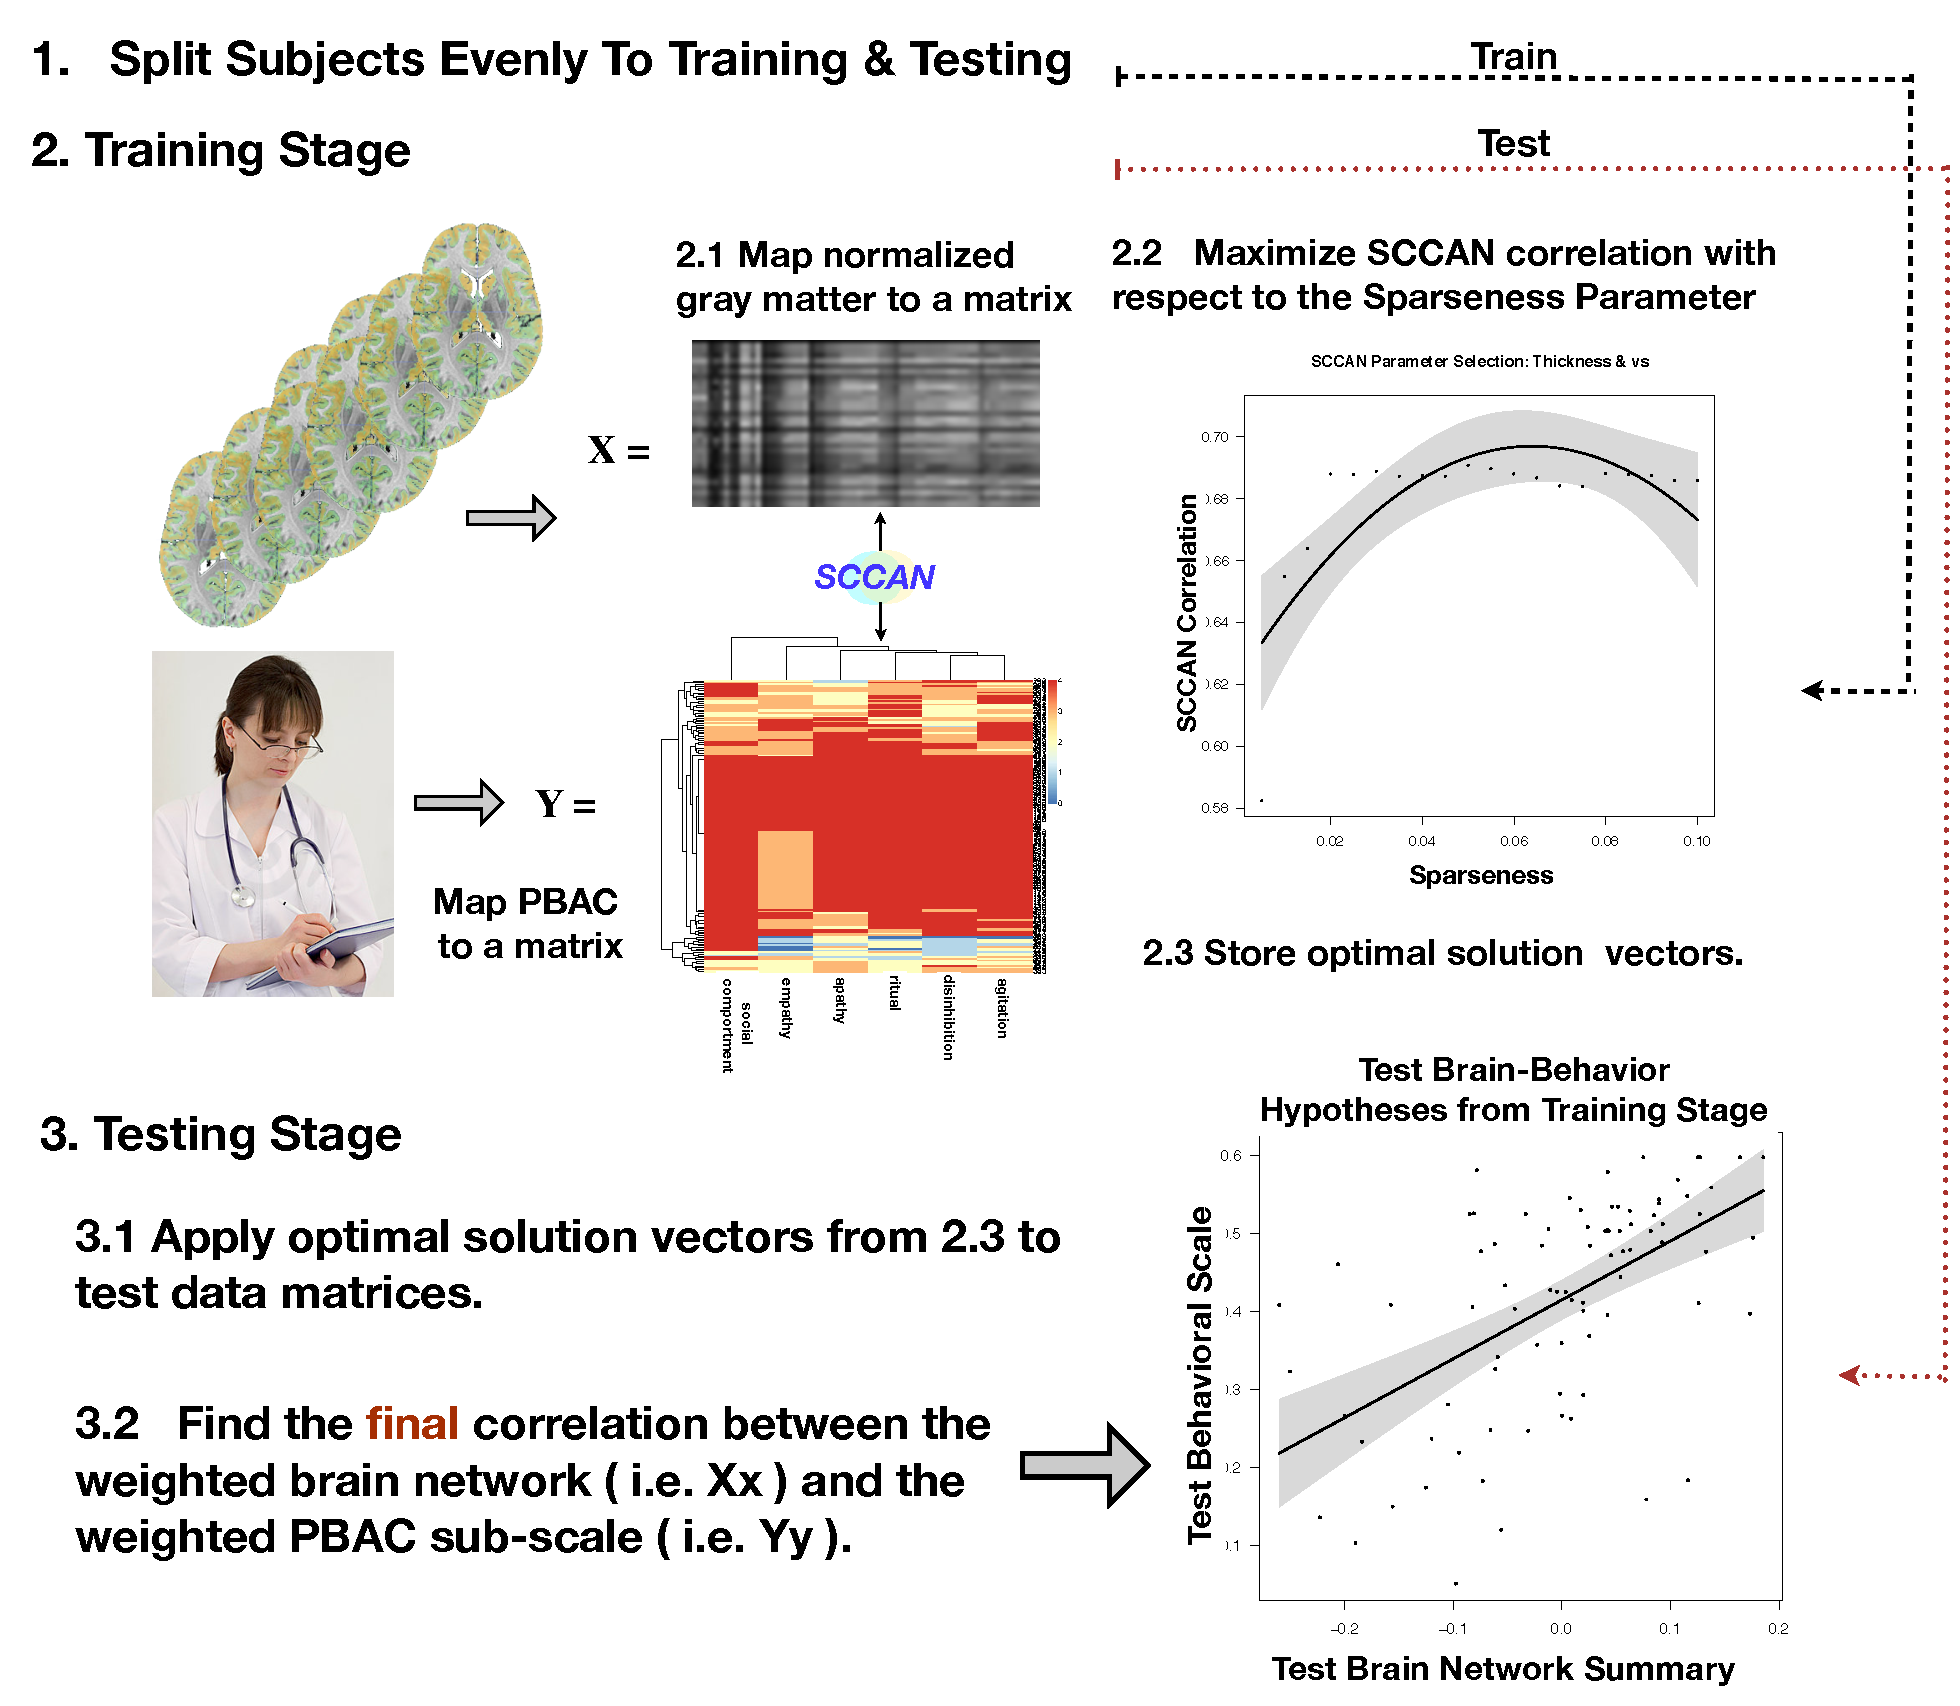
\includegraphics[width=0.9\textwidth]{./figs/sccan_study.pdf}
\caption{Diagram of the study.  The data splitting in step 1 happens only once.  We perform stage 2 and 3 for each of the five PBAC sub-scales.}
\label{fig:study}
\end{figure*}

\section{Methods} An overview of our study is in Figure~\ref{fig:study}.  We first discuss the core dataset and measurements.  We then discuss the PBAC and SCCAN methods.  We proceed with an evaluation framework, including a comparison against a univariate approach.
\subsection{Patients}  Individuals participating in the current research were drawn from a corpus of 270 patients, previously described \citet{libon_philadelphia_2011}.  Dementia patients were evaluated by experienced behavioral neurologists (AC, HBC, RGG, MG) and classified clinically on the basis of previously published criteria \citet{McKhann01,Rascovsky2011,Gorno-Tempini20111006}.  A research diagnosis was made on the basis of an independent review of a semi-structured history obtained from patients and their families and a detailed neurologic examination.  At least two trained reviewers from a consensus committee (inter-rater reliability, r= 0.91, p $<$ 0.001) confirmed patients' clinical diagnosis and presence of a specific dementia syndrome involving AD or FTLD. Discrepancies were resolved based on group discussion and follow-up assessment.  The PBAC was not used for the initial diagnosis of research participants.  

The clinical diagnosis of dementia was consistent with serum studies, clinical studies of cerebrospinal fluid (when available), clinical imaging studies such as MRI or CT, and functional neuroimaging studies such as SPECT or PET (these studies were not available to the consensus committee).  Exclusion criteria included the presence of other neurologic conditions such as stroke or hydrocephalus, primary psychiatric disorders (e.g., major depression, psychosis), or a systemic illness that can interfere with cognitive functioning.  Some patients were taking a cholinesterase inhibitor (e.g. donepezil, galantamine), memantine, or a non-sedating anti-depressant (e.g., serotonin-specific re-uptake inhibitors such as sertraline), or an atypical neuroleptic agent (e.g., quetiapine) consistent with clinical care; however, no patient demonstrated evidence of sedation.  The current research examined patients with AD (n= 17), behavioral variant-FTD (bvFTD; n= 41), semantic variant-primary progressive aphasia (svPPA; n= 14), non-fluent/ agrammatic-primary progressive aphasia (nfaPPA; n= 15) and corticobasal syndrome (CBS; n= 24).  The imaging analysis also included elderly controls (n= 56) who were living independently in the community and not taking psychoactive medications.  Normal control participants presented with no cognitive complaints or impaired instrumental activities of daily living.  Table 1 summarizes participant demographic features.  This research was approved by the University of Pennsylvania Institutional Review Board and informed consent was obtained consistent with the Declaration of Helsinki.

\input{src/demog.txt}

\subsection{The Philadelphia Brief Assessment of Cognition (PBAC)} Full details regarding the rationale and construction of the PBAC can be found elsewhere \citet{libon_philadelphia_2011}.  The PBAC consists of 20 variables grouped into 5 domain-specific rating scales.  These variables are grouped into five sub-scales measuring: working memory/ executive control, language, visuospatial/ constructional ability, verbal/ visual episodic memory, and behavior/ social comportment.  The total PBAC score ranges between 0-93. 
The executive scale includes measurements of fluency, digits backward and digits forward.  The language scale measures naming, speech, reading, writing and semantic ability.  The memory scale quantifies delayed free recall, recognition and Rey recall.  The visuospatial scale measures judgement of line orientation (JOLO) and the Rey copy test.  The behavioral scale includes subjective measurements of apathy, disinhibition, social comportment, agitation, empathy and ritual.   The correlations between these different sub-scales are shown in Figure~\ref{fig:pbaccor}.  

\begin{figure*}[th] \centering
\includegraphics[width=0.9\textwidth]{figs/pbac_correlations.pdf}
\caption{We visualize, with a heatmap, the correlations between the different PBAC individual scales which are clustered together to form the sub-scales studied here.  The total PBAC is an average of the 5 sub-scale scores.  The sub-scales provide a reasonable separation of measurements.}
\label{fig:pbaccor}
\end{figure*}

\subsection{Image acquisition}  All images were acquired with a Siemens Trio 3.0 tesla MRI scanner.  Following a rapid sagittal T1-weighted scan to determine patient position, a T1-weighted structural image was acquired with TR= 1620ms, TE= 3ms, slice thickness= 1mm, in-plane resolution= 0.9766mm $\times$  0.9766mm, FOV= 256 $\times$ 192. 

\subsection{Image processing} 

The imaging analysis is based on the publicly available and open-source Advanced Normalization Tools (ANTs, \url{stnava.github.io/ANTs/}) and the associated pipelining framework PipeDream (\url{http://neuropipedream.sourceforge.net}).  PipeDream automates and quality-assures ANTs processing via a single parameter file and data organization hierarchy.  Each patient's T1 imaging data are inhomogeneity corrected via the N4 bias correction algorithm \citet{Tustison2010}.  PipeDream then performs diffeomorphic normalization via the top-performing symmetric normalization methodology available in ANTs \citet{Avants2008,Avants2011a,wbir2012,Tustison2012} to map each subject to a population-specific template built from the same scanner and imaging parameters.  The template contains prior labeling and probability maps that are used to guide both brain extraction and neuroanatomical segmentation.  Segmentation is performed with a Markov Random Field approach \citet{Avants2011} implemented in the ANTs toolkit which has been validated on publicly-available datasets.  GM probability maps are then smoothed by a 2mm Gaussian kernel, mapped to the template space, and down-sampled to 2mm resolution.  These normalized GM probability maps are used for subsequent multivariate correlation with PBAC.

\subsection{Dimensionality reduction/Statistical Analysis} 

There are two primary reasons that univariate approaches lack power.  First, power is compromised because the same test is repeated at each measurement site leading to an often severe multiple comparisons problem.  Second, univariate methods do not exploit the latent signal in the data that is spread across measurement sites.  In this study, rather than perform voxel-wise testing, we employ a dimensionality reduction method implemented in SCCAN.  Briefly, this is an imaging-specific extension of sparse canonical correlation analysis \citet{Avants2010,Cao2009,parkhomenko,witten_extensions_2009-1,witten} that is itself a sparse extension to Hotelling's seminal canonical correlation analysis (CCA) \citet{Hotelling1936,hotellingcca}.  CCA, in turn, is a multi-modality extension to  principal component analysis. 

Classical CCA may be used to compute a multivariate association between two different views of a dataset.  One of Hotelling's original examples associated measurements of height and weight to measurements of cognition.  More recently, sparse versions of CCA have been developed to increase the interpretability of the output where we take motivation for sparse methods from our introductory material.  Sparse CCA methods, like classical CCA, compute eigenvectors (in actuality, {\em pseudo}-eigenvectors) that maximize the Pearson correlation between the input modalities.\footnote{Pseudo-eigenvectors are based on optimizing an objective function that is related to the eigenvalue problem but may not strictly satisfy the eigenvalue problem and related constraints}.  In this work, we use sparse CCA in a similar way to Hotelling's classic study, i.e. to associate two different types of measurements, one anatomical and one psychometric, in a population.

We employed the SCCAN implementation of sparse CCA to directly associate the five PBAC sub-scales described above with GM measures taken from T1-weighted MR images.   In general, SCCAN elucidates the relationship between two sets of measurements taken across a population and is thus well-suited to multivariate neuroimaging data.  The input to SCCAN is two matrices $X$ and $Y$.  The size of $X$ is $n \times p$ where $n$ is the number of subjects and $p$ is the number of voxels from the cortical gray matter.  The matrix thus collects all cortical imaging data for each subject.  The size of $Y$ is $n \times q$ where there are $q$ psychometric measurements in the given PBAC sub-scale i.e. $q=3$ for executive, $5$ for language, $3$ for memory, $2$ for visuospatial and $6$ for behavioral scales \footnote{One column of the behavioral scales (self insight) was excluded due to lack of variance}.  SCCAN maximizes the Pearson correlation, in a rotated space, between non-negatively weighted columns of these matrices.   More formally, SCCAN,  like classic CCA, introduces new unknown solution vectors, $x$ ( $p \times 1$ ) and $y$ ( $q \times 1$ ) that act as weight functions on columns of $X$, $Y$.   The SCCAN optimization criterion is: 
%
%                                         arg max   Corr( X x, Y y)  -  w || x ||  - v || y ||, 
%			     subject to:    x  >= 0,
%
\begin{eqnarray} 
\label{eq:cca}
 x^\star,~y^\star  =
\underset{x,y}{\operatorname{arg\,max}} \quad~
 ~~\frac{x~X^T ~Y~y}{\| X x \|~\| Y y \|}~\\ \notag \text{subject to} \\ \notag \sum_j
\|x^j\|_1 \leq s,~~ x^j \ge 0,
\end{eqnarray} where $x^\star$, $y^\star$ are the optimal solution vectors, $x^j$ denotes the $j^\text{th}$ entry of $x$, $s$ determines the sparseness level and $\|\cdot\|_1$ denotes the $\ell_1$ norm. The $\ell_1$ norm forces the solution $x$ to be sparse i.e. have zero value over the majority of the brain.  In this application, we do not enforce sparseness on the $y$ vector as it is relatively small, i.e. $q << n$.  SCCAN's objective function can be optimized even when the matrices are “fat” i.e. $p >> n$, often the case in neuroimaging studies.  Due to the non-linear (even np-hard) nature of subset selection (sparse optimization) from a large matrix, optimizing for a single canonical variate pair, $x, y$, involves a nonlinear gradient descent on the objective function above. 
The analytical gradient of the objective function (ignoring the $\ell_1$
and positivity constraints) w.r.t. $x$ is:
\begin{gather}
\label{eq:ccagrad}
X^T Y y - \frac{1}{2} X^T X x \| X x \| \| Y y \|. 
\end{gather}
Following this gradient will cause the candidate solution $x$ to leave the
permissible solution space and, as such, we follow the gradient update
step with a projection step as in
\citet{Polak1997,schwartz_family_1997}.  The projection step involves a
standard soft-thresholding operation used in $\ell_1$ optimization
which is easily modified to include positivity constraints
\citet{donoho_-noising_1995,tibshirani_regression_1996,elad_why_2006,witten_extensions_2009-1}.
The gradient for $y$ is obtained at the same time as that for $x$ with a simple switching of
variables.  Following, we refer to $x^\star$ as $x$ and $y^\star$ as $y$ interchangeably.  

SCCAN therefore produces a sparse projection vector acting on GM voxels that, taken as a set, maximally correlate with the user-selected PBAC domain of interest.  Here we use the working memory/executive, language, visuospatial, memory, and social/behavioral PBAC sub-scales, thus requiring only five direct multivariate tests, i.e., one for each cognitive domain.  The sparse eigenvectors that emerge from SCCAN identify the brain regions supporting the specific PBAC domain that was passed to the algorithm as the second view.  In this study, we restrict the SCCAN eigenvectors to be positive.  Thus, each eigenvector can be reinterpreted as a weighted average of values over a restricted region of GM, like a region of interest \citet{roi_analysis,zhou_hierarchical_2011,Rasmussen2012,Chen2010}.  This may be achieved in a post-processing step that sets the sum of the solution vector, $x$ or $y$, to equal one.  The implementation details are available in the Advanced Normalization Toolkit's \verb sccan.cxx ~program which contains the SCCAN source code.  The significance of SCCAN results may be tested by permuting one of the two views over many different simulations.  One then compares the correlation value produced by the original ordering of the data to the correlations produced over the $N$ permutations. Large $N$ (typically $>1000$) is needed to provide a reasonable sampling of the empirical null distribution.  In this analysis, we use a training and testing paradigm \footnote{as recommended by reviewers} to avoid permutation testing and to allow us to perform parameter selection (for $s$) on the training dataset in a manner that is independent of the test dataset. 

\begin{figure*}[th] \centering
\includegraphics[width=0.18\textwidth]{./figs/sccan_param_behav.pdf}
\includegraphics[width=0.18\textwidth]{./figs/sccan_param_exec.pdf}
\includegraphics[width=0.18\textwidth]{./figs/sccan_param_lang.pdf}
\includegraphics[width=0.18\textwidth]{./figs/sccan_param_mem.pdf}
\includegraphics[width=0.18\textwidth]{./figs/sccan_param_vs.pdf}
\caption{A one parameter search over sparseness, in the training dataset, allows us to identify the optimal sparseness parameter for each cognitive domain.  The network variables $x^\star$ and $y^\star$ that arise from SCCAN computed at the optimal sparseness level will be evaluated in the test dataset for reproducibility.}
\label{fig:param}
\end{figure*}

\subsection{Parameter Selection}  
\subsubsection{Image Processing}
Our studies used reproducible research practices by employing open methods, standardized parameter sets and version control of both parameters and code via git.  We employed standard parameters in PipeDream and ANTs for template construction, normalization, segmentation and GM estimation.  These analysis protocols are described elsewhere \citet{Avants2011a,Avants2011,Tustison2012,Tustison2010}. 

\subsubsection{Statistical Parameters}
SCCAN was used to extract the single most dominant features associating GM and a PBAC sub-scale in a training dataset.  Our study design involves setting only a single parameter, $s$, which controls the sparseness of the imaging space solution vector, $x$.  We chose to restrict $x$ to also be non-negative such that the solutions can be interpreted with clear directionality i.e. as a weighted average.  To identify the parameter $s$, we run SCCAN with a range of $s^{\text{candidate}}$ values ($s=0.005,0.01,\cdots,0.5)$ and store the resulting SCCAN correlation for each trial.  We then fit a model, $ \text{SCCAN-Correlation} \approx   \beta_1 s^{\text{candidate}} + \beta_2 ( s^{\text{candidate}} )^2 +  \beta_3 ( s^{\text{candidate}} )^3 + \beta_4 ( s^{\text{candidate}} )^4$, to the function mapping $s \to $ SCCAN-Correlation.  We set the the final parameter $s$ to correspond to the value of our model that maximizes the dependent SCCAN-Correlation value.  If there are ties, we take the first from the left (maximally sparse) solution.   We then compute the final solutions $x^\star, y^\star$ that will be evaluated for reproducibility in our test dataset.  We did not employ sparseness on the 2nd view (the PBAC sub-scale scores).  In total, we need only perform $5$ tests total as opposed to 5$p$ tests required by a univariate setting.  Here, $p=90,084$ and $5p=450,420$.  Parameter selection results are in Figure~\ref{fig:param}.

\subsection{Comparison of Univariate to Multivariate Feature Selection}
This study employs a training and testing paradigm.  Therefore, SCCAN may be viewed as a tool that generates ``feature vectors" ($x, y$) that are optimized in a multivariate manner to associate GM and PBAC.  Using our existing terminology, these maximize $Corr( X x  , Y y )$ where $Corr$ denotes Pearson correlation and $X, Y$ correspond to the training dataset matrices.  
These feature vectors may be used as ``hypotheses" and applied to a new testing dataset, $X_\text{test}, Y_\text{test}$, to determine if the patterns extracted from training data are reliable in test data.  In this analysis, we use the correlation in test data as our outcome measurement which is computed as $\text{Outcome}_\text{Multivariate}=Corr( X_\text{test} x, Y_\text{test} y )$ where $x, y$ derive from training data. 


% \begin{figure*}[th] \centering
% \includegraphics[width=0.9\textwidth]{./figs/results.pdf}
% \caption{...}
% \label{fig:results}
% \end{figure*}

We can also compute a parallel univariate outcome, $\text{Outcome}_\text{univariate}$, via a similar methodology based on univariate feature selection.  We use Occam's razor to decide upon a univariate feature selector i.e. we do something simple-minded yet akin to several other studies \citet{Chen2010,dickerson_mri_2012}.  We compute the univariate p-values of a model associating the PBAC sub-scale summary measurement (an average of the $Z$ transformations of the individual measurements within the sub-scale) with each voxel in the cortex.  This univariate model may be written PBAC-sub-scale $\approx v_i$ where $v_i$ is a vector containing the subject GM values at a given voxel (so $i$ takes values $1 \cdots p$).  The p-value associated with $v_i$ is then denoted p$_i$.  Now, define $u$ as a $p$-length weight vector similar to the weight vector $x$.  However, the entry at $u_i$ is zero if p$_i$ is $>0.01$ (unadjusted) and 1 otherwise. This finally allows us to define the univariate outcome as $\text{Outcome}_\text{univariate}=Corr( X_\text{test} u , \text{PBAC-sub-scale}_\text{test} )$.   

This protocol allows us to compare a joint multivariate feature selector that identifies weights on PBAC sub-scale values ($y$) and the brain ($x$) with a univariate feature selector acting only on the brain ($u$).  While the univariate approach does not weight the PBAC-sub-scale, it does use a standard average of the sub-scales commonly used in PBAC assessment.  Thus, we compare a new, fully multivariate approach, to an existing standard approach.  One may argue that the threshold selected to binarize the $u$ vector is arbitrary.  However, this is a common/standard style of analysis employed in univariate methods, i.e. select a significance threshold and accept the results as the truth.  The univariate solutions do not survive multiple comparisons correction so we had no choice but to use uncorrected p-values as feature selectors.


\begin{figure*}[th] \centering
\includegraphics[width=0.98\textwidth]{./figs/sccan_Ax.png}
\includegraphics[width=0.98\textwidth]{./figs/sccan_Sag.png}
\caption{All of the $x^\star$ solution vectors are combined in axial and sagittal views of the brain.  Red is behavior, blue executive, green language, magenta episodic memory and yellow visuospatial.}
\label{fig:slices}
\end{figure*}


\begin{figure*}[th] \centering
\includegraphics[width=0.22\textwidth]{./figs/sccanpredictbehav.pdf}
\includegraphics[width=0.25\textwidth]{./figs/ren_behav_anterior.png}
\includegraphics[width=0.25\textwidth]{./figs/ren_behav_lateral.png}
\includegraphics[width=0.22\textwidth]{./figs/pbac_image_behav}
\includegraphics[width=0.22\textwidth]{./figs/sccanpredictexec.pdf}
\includegraphics[width=0.25\textwidth]{./figs/ren_exec_anterior.png}
\includegraphics[width=0.25\textwidth]{./figs/ren_exec_lateral.png}
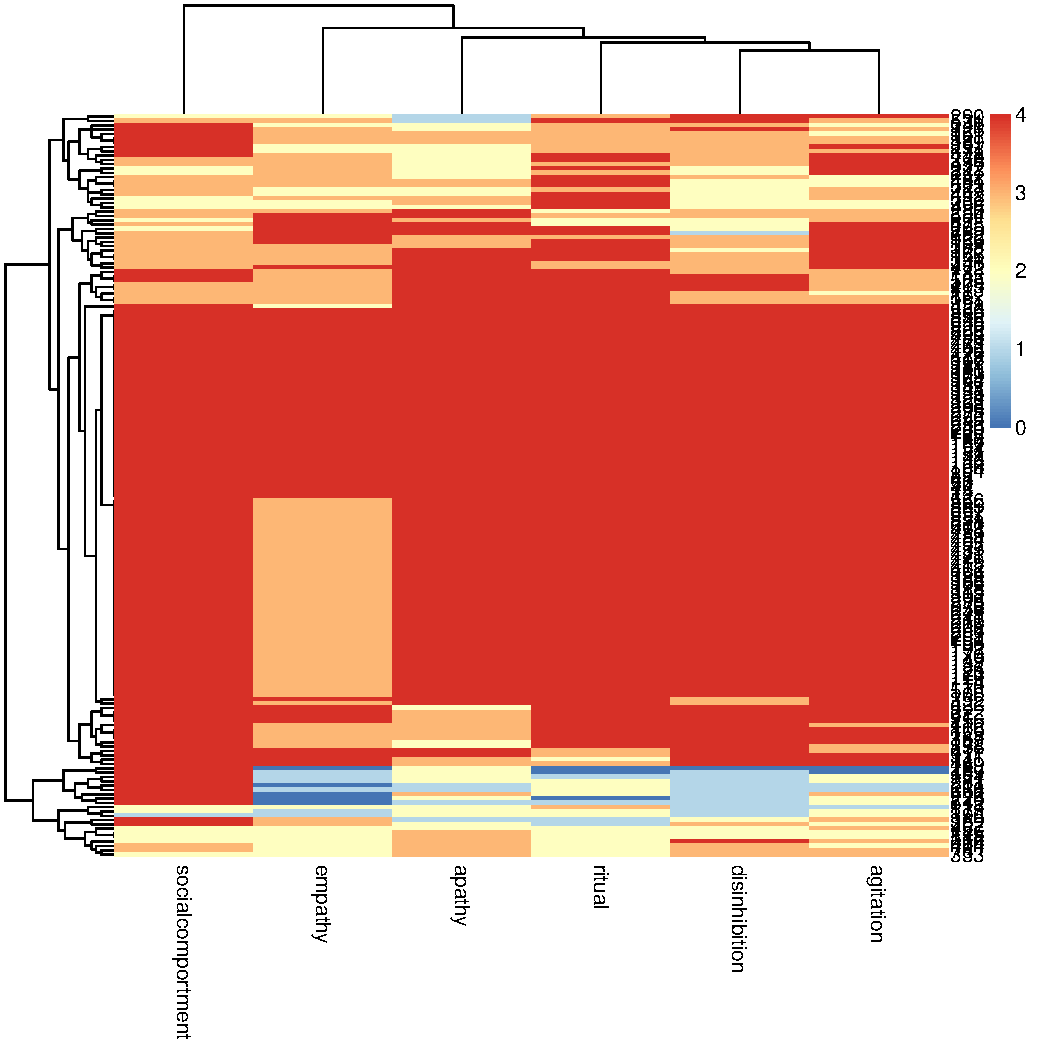
\includegraphics[width=0.22\textwidth]{./figs/pbac_image_exec}
\includegraphics[width=0.22\textwidth]{./figs/sccanpredictlang.pdf}
\includegraphics[width=0.25\textwidth]{./figs/ren_lang_anterior.png}
\includegraphics[width=0.25\textwidth]{./figs/ren_lang_lateral.png}
\includegraphics[width=0.22\textwidth]{./figs/pbac_image_lang}
\includegraphics[width=0.22\textwidth]{./figs/sccanpredictmem.pdf}
\includegraphics[width=0.25\textwidth]{./figs/ren_mem_anterior.png}
\includegraphics[width=0.25\textwidth]{./figs/ren_mem_lateral.png}
\includegraphics[width=0.22\textwidth]{./figs/pbac_image_mem}
\includegraphics[width=0.22\textwidth]{./figs/sccanpredictvs.pdf}
\includegraphics[width=0.25\textwidth]{./figs/ren_vs_anterior.png}
\includegraphics[width=0.25\textwidth]{./figs/ren_vs_lateral.png}
\includegraphics[width=0.22\textwidth]{./figs/pbac_image_vs}
\caption{We visualize the correlation between $X_\text{test} x^\star$ and $Y_\text{test} y^\star$ for each of the five PBAC sub-scales.  We also show the PBAC sub-scales and their corresponding putative support regions in the cortex, as identified by SCCAN and verified in testing data.
Each row, from the top, contains the results for the behavioral/social comportment scale, the executive/working memory scale, the language scale, the episodic memory scale and the visuospatial scale.}
\label{fig:test}
\end{figure*}

\begin{comment}
\begin{figure*}[th] \centering
\includegraphics[width=0.4\textwidth]{./figs/sccanpredictbehav.pdf}
\includegraphics[width=0.4\textwidth]{./figs/sccanpredictexec.pdf}
\includegraphics[width=0.4\textwidth]{./figs/sccanpredictlang.pdf}
\includegraphics[width=0.4\textwidth]{./figs/sccanpredictmem.pdf}
\includegraphics[width=0.4\textwidth]{./figs/sccanpredictvs.pdf}
\caption{We visualize the correlation between $X_\text{test} x^\star$ and $Y_\text{test} y^\star$ for each of the five PBAC sub-scales.}
\label{fig:test}
\end{figure*}
\end{comment}


\section{Results}

% We residualized the input matrices with respect to age, educational level (in years) and MMSE before 
%  sending them to the univariate and multivariate outcome procedure outlined in Figure~\ref{fig:study}.  

\subsection{Univariate: PBAC Sub-Scales and GM Density} No univariate outcome measurement achieves significance when relating brain and behavior in the test data.  That is, the correlation between PBAC-sub-scale$_\text{test}$ with $X_\text{test} u$ is weak in each of the five PBAC sub-scales (p-values: exec 0.93,  language 0.078,  memory 0.85, visuospatial 0.66, behavioral 0.78).  However, the relationship between PBAC-sub-scale$_\text{train}$ with $X_\text{train} u$ is strong, as expected (all p-value $< 0.01$).  This indicates that, at least in this dataset, naive univariate feature selection overfits to the training data.  

\subsection{Multivariate: PBAC Sub-Scales and GM Density}  
Based on training data, we found, in testing data, significant associations between GM density and each of the five PBAC sub-scales consistent with putative neuroanatomical substrates at the Bonferroni-corrected $p < 0.01$ level.  Scatterplots are in Figure~\ref{fig:test} where raw p-values are also reported (rounded below 0.0001 to 0).  Figure~\ref{fig:slices} shows the $x$ function for each sub-scale plotted on the brain.  Note these are {\em sparse} functions i.e. no additional thresholding is performed to generate these overlays.    Figure~\ref{fig:test} shows the test data relationship between brain and behavior, as well as a visualization (in heatmap form) of each PBAC sub-scale.  

\noindent {\em Reporting Multivariate Results:}  We display SCCAN {\em pseudo}-eigenvectors on the brain in a manner that is similar to traditional voxel-based analysis, as in Figure~\ref{fig:slices}.  As mentioned in the Methods section, these weight vectors are similar to weighted averages in that the difference between these vectors and a traditional weighted average is only a scalar multiplication.  Therefore, the effect on a correlation is null.  We also tabulate results in Talairach coordinates similar to traditional methods (e.g. Table~\ref{tab:behav}).  However, instead of plotting coordinates of peak p-values, we annotate the Talairach coordinate of each spatial component of the {\em pseudo}-eigenvector such that we gain a degree of spatial resolution in the interpretation of SCCAN results.  Despite using a familiar reporting system, the key point is that p-values are assessed over the relationships computed from the entire operation on the multivariate dataset (e.g. $Corr(X_\text{test} x^\star,Y_\text{test} y^\star)$).  Thus, we are reporting the collection of neuroanatomical data points that contribute to the relationship with cognition as opposed to a single point.  We estimate Brodmann areas and AAL labels from the label sets included with mricron \citet{Rorden2007a}.  Figure~\ref{fig:test} displays results in a glass brain where we draw connections between the major sub-regions of the pseudo-eigenvectors.  We also show, via a heatmap, the distribution of cognitive scores for each PBAC sub-scale.  Most importantly, we display the distribution of the test dataset gray matter against cognition.

As summarized in Figure~\ref{fig:test} and Table~\ref{tab:behav}, PBAC-defined behavior/social comportment focuses on medial and inferior prefrontal cortex.  The memory sub-scales (Table~\ref{tab:mem}) relates to precuneus, hippocampus, and bilateral posterior temporal atrophy more prominently on the left than the right.  Significant visuospatial/constructional impairment (Table~\ref{tab:vs}) relates to bilateral posterior temporal-occipital and bilateral parietal-occipital lobe.  The language sub-scale (Table~\ref{tab:lang}) was related to left temporal and left temporal-parietal gray matter.  The executive network involves a distributed temporal and frontal network and is described in Table~\ref{tab:exec}.  

\input{src/behav_network.txt}

\input{src/exec_network.txt}

\input{src/lang_network.txt}

\input{src/mem_network.txt}

\input{src/vs_network.txt}


\begin{comment}
\subsection{Clinical Diagnosis and GM Density} PBAC sub-scales have previously been shown to differentiate between AD and FTLD, and between FTLD phenotypes9,libon_philadelphia_2011.  Linear regression was used to relate GM density to the diagnosis of interest while controlling for co-variates including age, education, disease duration.  Here, diagnosis is a binary predictor where a single patient group was compared to all other subjects not in the group of interest.  Results confirm that the weighted average GM density associated with most PBAC sub-scale was significantly related to diagnosis.  Specifically, PBAC behavior/social-related GM regions were related to bvFTD (p< 0.001).  Likewise, PBAC language-related GM regions were related to svPPA (p< 0.008).  PBAC memory-related GM regions were related to AD (p< 0.017) and PBAC visuospatial/ constructional-related GM regions were related to CBS (p< 0.001).  PBAC working memory/ executive-related GM regions were not related to one specific clinical diagnosis.  
\end{comment}

\section{Discussion}
This study establishes, for the first time, that sparse canonical correlation analysis finds repeatable relationships between multivariate psychometric batteries and network level gray matter density measurements.  Our analysis restricts the signs of the gray matter density solution vector, $x^\star$, to be sparse and positive enabling directional relationships to be established (i.e. low gray matter, low cognitive score).  The SCCAN multivariate analysis framework shows improved generalizability and power over the univariate method against which it is compared.  

This study also represents the first comparison of PBAC sub-scales to structural neuroimaging. The PBAC was designed as a screening instrument to assess overall dementia severity and to differentiate between neurodegenerative syndromes within the AD and FTLD spectrum.  Previous research with the PBAC found a significant correlation between the total PBAC score and the MMSE \citet{Libon2007,libon_philadelphia_2011}, thus demonstrating that performance on the instrument reasonably captures overall dementia severity. The psychometric qualities of the PBAC include good internal consistency among the tests within each PBAC sub-scale and highly significant intra-class correlations between PBAC sub-scales and standard neuropsychological tests \citet{libon_philadelphia_2011}.  PBAC sub-scales also show good clinical utility in distinguishing between AD and FTLD, and between FTLD-related phenotypes using sub-scale cut scores, although diagnosis is not the focus here. 

The current research used novel imaging methods to provide further evidence for the criterion validity of the PBAC by associating PBAC sub-scale test performance with corresponding areas of GM atrophy.  The heterogeneity of this population (which includes controls and five different clinical phenotypes) drives these relationships.  For instance, patients with AD are known to present with striking memory impairment as well as atrophy involving the hippocampus, precuneus and related anatomic structures.  In the current research, the PBAC memory sub-scale was associated with GM involving left hippocampus tail, hippocampus mid-body and precuneus.   Hippocampal and precuneus involvement in clinically-defined patients with anterograde amnesia and AD is well known \citet{Nestor2002b,Pengas2010}.  Moreover, prior research with AD and amnesic mild cognitive impairment suggests that these areas are part of a neurocognitive network for memory that also includes superior temporal gyrus \citet{Delano-Wood2012,Gardini2011}.  Table~\ref{tab:mem} shows all regions associated by SCCAN to the verbal and visual episodic memory sub-scale. 

The behavioral variant of FTLD induces variance in the behavioral sub-scale.  bvFTLD presents with alterations in social comportment \citet{Rascovsky2011,Shany-Ur2011}, including apathy, disinhibition, and lack of empathy.  In the current study, the PBAC-behavior/social scale is related to striking bilateral medial and ventral frontal GM, perhaps with greater right-sided involvement.  Previous research has associated these behavioral abnormalities with bilateral ventral and medial frontal atrophy \citet{Massimo2009,Rosen2010}.  

Similarly, CBS is associated with significant impairment in visuospatial and visuoconstructional tests, as well as some executive deficits \citet{Libon2007,Libon2009}.  The current research associates the PBAC-visuospatial/constructional sub-scale with right posterior GM atrophy including parietal and occipital lobes.  Prior neuroimaging research with CBS patients is controversial, with some researchers suggesting both parietal and frontal atrophy \citet{Grossman2004b} and others only frontal involvement \citet{Hassan2011}.  In the present study, atrophy in primarily right visual association cortex was related to the visuospatial/constructional sub-scale which, in turn, was designed to identify individuals with the clinical diagnosis of CBS.  Table~\ref{tab:vs} highlights the visuospatial network defined by SCCAN.

In contrast to other domains, the executive/ working memory sub-scale is not typically associated with a single diagnosis but instead is associated with several diagnostic subgroups, including CBS, bvFTLD and AD.  Prior research with the PBAC has shown that patients with naPPA score lower on the PBAC-working memory/executive sub-scale \citet{libon_philadelphia_2011,Libon2007} confirming executive and working memory deficits in these patients and reflecting their disease centered primarily in the frontal lobe \citet{Gunawardena2010,Rogalski2011}.  The executive network highlights diverse regions (see Table~\ref{tab:exec}) including superior temporal gyrus which has been previously implicated as a neural substrate for the digits backward test \citet{Li2012}.  Inspecting Figure~\ref{fig:slices} shows the executive scale extracts several brain regions that form key points in the default mode network such as precuneus, superior prefrontal cortex, lateral temporal lobe and lateral superior parietal cortex \citet{Buckner2008}.  The PBAC-working memory/executive sub-scale consists of verbally-mediated tests and, as such, several language regions are involved as well.  

The PBAC language sub-scale is strongly related to left temporal GM density, primarily with prominent posterior and inferior temporal GM.  These data are consistent with prior research demonstrating left temporal atrophy in patients with svPPA who have language-related cognitive impairment \citet{Bonner2009,Williams20051042}.  The measures on the PBAC language sub-scale focus mostly on object comprehension, single word expression, reading and writing, with little emphasis on the characteristics important for identifying naPPA \citet{Gorno-Tempini20111006}.  Future modifications of the PBAC may include measures to improve detection of regions that would be specifically impaired in the naPPA subgroup.  Such focused tests are not currently included in PBAC.


Taken together, these data extend past research to show that PBAC sub-scales are associated with MRI-defined anatomical substrates.  The identified relationships between neurocognitive GM networks and psychometrics underscores the power of SCCAN over traditional univariate approaches to imaging analysis.  By using SCCAN, we obtain massive dimensionality reduction which significantly enhances the empirical ability to detect these behavioral and neuroimaging relationships in both training and testing data.  Prior work demonstrated the advantages of SCCAN in combining GM and diffusion tensor imaging data to distinguish between autopsy- and CSF-defined cases of AD and FTLD \citet{Avants2010b}.  The results of the current study reveal that SCCAN is capable of associating multi-dimensional psychometric and neuroimaging data to reveal the large-scale neural networks that are degraded when cognition is compromised in neurodegenerative conditions like AD and FTLD.

There are several caveats to this study.  A primary technical issue is whether the network structure (i.e. distributed sets of voxels) that SCCAN extracts is either a minimal or maximal reliable network supporting the selected cognitive domain.  Indeed, it is likely that subsets of the voxels added to or subtracted from the SCCAN solutions may not alter predictive accuracy to a strong degree.  This hypothesis is strengthened by the fact that our sparseness versus correlation curves ( Figure~\ref{fig:param} ) are relatively smooth. However, identifying an optimally predictive set of high-dimensional variables across arbitrary subsets of a population is a generally unsolved problem.  We elected to address this by defining our networks based on a tractable parameter search strategy that maximizes the SCCAN correlation in training data.  A secondary issue is that our comparison with the univariate strategy may not be ideal.  There are several alternative approaches for univariate feature selection that may be employed with better results, for instance optimizing the recently proposed cluster-level FDR \citet{Chumbley2009}.  We leave this question to future work by ourselves or others and also note that this approach would remain univariate in the dependent variable.  SCCAN, on the other hand, uses a multivariate treatment of both datasets, cognition and neuroimaging.

The clinical aspects of this research also has limitations.  First, the PBAC was not designed nor should it be used to as a substitute for a comprehensive neuropsychological evaluation. This is reflected most clearly in the fact that PBAC sub-scales appear to extract primarily posterior temporal regions, medial frontal regions, medial posterior regions and parietal lobe.  There is little representation of motor regions and anterior temporal regions.  Second, the sample size for several groups was relatively modest which makes evaluating diagnostic power very challenging due to the large number of diverse phenotypes, i.e. 5 neurodegenerative and one control group.  The results of the present study will require confirmation with larger groups of patients.  Further evaluation of SCCAN as a tool to aid diagnosis and prognosis are also required.  Third, virtually all work with the PBAC has been confined to differentiating AD from FTLD and to distinguishing between FTLD phenotypes.  The utility of the PBAC in other populations such as Parkinson's disease, amyotrophic lateral sclerosis, and Mild Cognitive Impairment requires further examination.  Finally, SCCAN associated some unexpected brain regions with a specific cognitive domain.  Additional work is needed to understand the basis for these associations and whether these additional voxels are part of a minimal or maximal predictive network.  With these limitations in mind, the current study suggests the power of a multivariate analytic approach such as SCCAN to interrogate multivariate brain and behavior relationships.  

\section{Acknowledgements}
Dr. Grossman receives support from the National Institutes of Health (AG32953, AG17586, AG15116, NS44266, and NS53488) and the Wyncote Foundation, and is a consultant for Bristol Meyers Squibb and Allon Therapeutics.  Dr. Chatterjee receives support from National Institutes of Health (RO1 DC008779, RO1 HD050199] and the National Science Foundation (SBE0541957).  Dr. McMillan receives support from NIH HD0406.  Ms. Massimo receives support from National Institutes of Health (F31NR013306) and John A. Hartford Foundation's Building Academic Geriatric Nursing Capacity Award Program.  Dr. Libon receives support for Bayer Pharmaceuticals.  Drs. Rascovsky and Avants, and Ms. Boller report no disclosures.

\section{ANTsR Example Code for SCCAN}

We first load the relevant libraries for this analysis.

\begin{knitrout}
\definecolor{shadecolor}{rgb}{0.969, 0.969, 0.969}\color{fgcolor}\begin{kframe}
\begin{alltt}
\hlfunctioncall{suppressPackageStartupMessages}(\hlfunctioncall{library}(ANTsR))
\hlfunctioncall{library}(xtable)
\hlfunctioncall{library}(abind)
\hlfunctioncall{library}(grDevices)
\hlfunctioncall{library}(visreg)
\hlfunctioncall{library}(vegan)
\end{alltt}
\end{kframe}
\end{knitrout}


Several organizational steps are not included.  The key steps of univariate and multivariate feature selection, along with assessment on testing data, are shown below. 




\begin{knitrout}
\definecolor{shadecolor}{rgb}{0.969, 0.969, 0.969}\color{fgcolor}\begin{kframe}
\begin{alltt}

\hlfunctioncall{if} (\hlfunctioncall{length}(resUV) != 5 & FALSE) \{
\hlcomment{    # do the univariate test to get the sparseness param}
    \hlfunctioncall{print}(\hlstring{"UNIVARIATE"})
    voxside <- \hlstring{" ~ vox "}
    \hlfunctioncall{if} (nam == \hlstring{"exec"}) 
        myform <- \hlfunctioncall{as.formula}(\hlfunctioncall{paste}(unames[1], voxside))
    \hlfunctioncall{if} (nam == \hlstring{"lang"}) 
        myform <- \hlfunctioncall{as.formula}(\hlfunctioncall{paste}(unames[2], voxside))
    \hlfunctioncall{if} (nam == \hlstring{"vs"}) 
        myform <- \hlfunctioncall{as.formula}(\hlfunctioncall{paste}(unames[3], voxside))
    \hlfunctioncall{if} (nam == \hlstring{"mem"}) 
        myform <- \hlfunctioncall{as.formula}(\hlfunctioncall{paste}(unames[5], voxside))
    \hlfunctioncall{if} (nam == \hlstring{"behav"}) 
        myform <- \hlfunctioncall{as.formula}(\hlfunctioncall{paste}(unames[6], voxside))
    \hlfunctioncall{print}(myform)
    bynum <- 1
    ss <- \hlfunctioncall{seq}(1, \hlfunctioncall{ncol}(trainmat), by = bynum)
    ntests <- \hlfunctioncall{length}(ss)
    progress <- \hlfunctioncall{txtProgressBar}(min = 0, max = ntests, style = 3)
    upvs <- \hlfunctioncall{rep}(1, \hlfunctioncall{ncol}(trainmat))
    \hlfunctioncall{for} (i in ss) \{
        vox <- trainmat[, i]
        fit <- \hlfunctioncall{lm}(myform, data = demog[permutesubs, ])
        upvs[i] <- \hlfunctioncall{coefficients}(\hlfunctioncall{summary}(fit))[2, 4]
        \hlfunctioncall{if} (i%%1000 == 0) \{
            \hlfunctioncall{setTxtProgressBar}(progress, i)
        \}
    \}
    sigthresh <- 0.01
    \hlfunctioncall{print}(\hlstring{""})
    sigfrac <- \hlfunctioncall{sum}(upvs < 0.05, na.rm = T)/ntests * 5
    upvs[\hlfunctioncall{is.na}(upvs)] <- 1
    qvsm <- upvs
    qvsm[upvs < sigthresh] <- 1
    qvsm[upvs >= sigthresh] <- 0
    qvsm <- qvsm/\hlfunctioncall{sum}(qvsm)
    qvsm <- \hlfunctioncall{matrix}(qvsm, nrow = 1)
    vox <- testmat %*% \hlfunctioncall{t}(qvsm)
    fit <- \hlfunctioncall{lm}(myform, data = demog[permutesubs2, ])
    \hlfunctioncall{print}(\hlfunctioncall{summary}(fit))
    uvimg <- \hlfunctioncall{antsImageClone}(maskimg)
    uvimg[mask] <- (1 - upvs)
    \hlfunctioncall{antsImageWrite}(uvimg, \hlfunctioncall{paste}(DIR, nam, \hlstring{"_uv.nii.gz"}, sep = \hlstring{""}))
    resUV <- \hlfunctioncall{lappend}(resUV, \hlfunctioncall{c}(nam, \hlfunctioncall{coefficients}(\hlfunctioncall{summary}(fit))[2, 4]))
\}  \hlcomment{# resUV length}
\hlcomment{# now do the multi-variate equivalent}
\hlfunctioncall{print}(\hlfunctioncall{paste}(\hlstring{"MULTIVARIATE "}))
clustthresh <- 100
\hlfunctioncall{if} (\hlfunctioncall{length}(sparMV) < 5) \{
    sparlist <- (\hlfunctioncall{seq}(1, 50, by = 4)/100)
    corrlist <- \hlfunctioncall{list}()
    \hlfunctioncall{for} (sigfrac in sparlist) \{
        \hlfunctioncall{print}(\hlfunctioncall{paste}(\hlstring{"SEARCH:"}, sigfrac))
        ff <- \hlfunctioncall{sparseDecom2}(inmatrix = \hlfunctioncall{list}(trainmat, cogmat[permutesubs, nw]), 
            inmask = \hlfunctioncall{c}(maskimg, NA), sparseness = \hlfunctioncall{c}(sigfrac, -1), nvecs = 1, 
            its = 1, cthresh = \hlfunctioncall{c}(clustthresh, 0), perms = 0, uselong = 0, z = 0, 
            smooth = 1, robust = 1)
        myproj1a <- trainmat %*% \hlfunctioncall{t}(\hlfunctioncall{imageListToMatrix}(ff$eig1, maskimg))
        myproj1b <- cogmat[permutesubs, nw] %*% \hlfunctioncall{as.matrix}(ff$eig2)
        corrlist <- \hlfunctioncall{lappend}(corrlist, \hlfunctioncall{cor.test}(myproj1a, myproj1b)$est)
    \}
    corrlist <- \hlfunctioncall{unlist}(\hlfunctioncall{unlist}(corrlist))
    fit <- \hlfunctioncall{lm}(corrlist ~ sparlist + \hlfunctioncall{I}(sparlist^2) + \hlfunctioncall{I}(sparlist^3) + \hlfunctioncall{I}(sparlist^4))
    \hlfunctioncall{pdf}(\hlfunctioncall{paste}(\hlstring{"figs/sccan_param_"}, nam, \hlstring{".pdf"}, sep = \hlstring{""}))
    mytitle <- \hlfunctioncall{paste}(\hlstring{"Correlation v. Sparseness "}, nam, sep = \hlstring{""})
    \hlfunctioncall{visreg}(fit, main = mytitle, xlab = \hlstring{"Sparseness"}, ylab = \hlstring{"SCCAN correlation"}, 
        cex.main = 2, cex.lab = 2)
    \hlfunctioncall{dev.off}()
    sigfrac <- sparlist[\hlfunctioncall{which}(corrlist == \hlfunctioncall{max}(corrlist))]
    sp <- \hlfunctioncall{data.frame}(sparlist = (\hlfunctioncall{c}(1:200)/1000))
    pc <- \hlfunctioncall{predict}(fit, newdata = sp)
    sigfrac <- sp$sparlist[\hlfunctioncall{which.max}(pc)]
    sparMV <- \hlfunctioncall{lappend}(sparMV, sigfrac)
\} else sigfrac <- sparMV[[opt]]
ff <- \hlfunctioncall{sparseDecom2}(inmatrix = \hlfunctioncall{list}(trainmat, cogmat[permutesubs, nw]), inmask = \hlfunctioncall{c}(maskimg, 
    NA), sparseness = \hlfunctioncall{c}(sigfrac, -1), nvecs = 1, its = 15, cthresh = \hlfunctioncall{c}(clustthresh, 
    0), perms = 0, uselong = 0, z = 0, smooth = 1, robust = 1)
myproj1a <- trainmat %*% \hlfunctioncall{t}(\hlfunctioncall{imageListToMatrix}(ff$eig1, maskimg))
myproj1b <- cogmat[permutesubs, nw] %*% \hlfunctioncall{as.matrix}(ff$eig2)
myproj2a <- testmat %*% \hlfunctioncall{t}(\hlfunctioncall{imageListToMatrix}(ff$eig1, maskimg))
myproj2b <- cogmat[permutesubs2, nw] %*% \hlfunctioncall{as.matrix}(ff$eig2)
cogweights <- \hlfunctioncall{c}(\hlfunctioncall{round}(ff$eig2 * 1000)/1000)
\hlfunctioncall{print}(cogweights)
imaging <- myproj2a[, 1]
cognition <- myproj2b[, 1]
myform <- \hlfunctioncall{as.formula}(\hlstring{" cognition ~ imaging "})
fit <- \hlfunctioncall{lm}(myform, data = demog[permutesubs2, ])
mypv <- \hlfunctioncall{coefficients}(\hlfunctioncall{summary}(fit))[2, 4]
\hlfunctioncall{print}(\hlfunctioncall{summary}(fit))
\end{alltt}
\end{kframe}
\end{knitrout}


\bibliographystyle{plainnat}
\bibliography{src/cca}
\end{document}
